\def\format{complete}

\part{关于WordHelper的说明文档}
\label{wordhelper}

\chapter{基础问题:}
\label{}

\section{WordHelper 是什么 ?}
\label{wordhelper}

回答: WordHelper是一款自主研发的app,它可以帮助你轻松愉快地学习英语。WordHelper 可以在windows, mac和linux上运行,目前它是基于命令行运行的。

\section{WordHelper 可以做什么?}
\label{wordhelper}

回答: WordHelper 旨在帮助您更加轻松愉快地学习英语。你可以用它来搜索单词,记录个性化的笔记,制定适合您的背单词方式,解析英文文本。

\section{从哪获得WordHelper?}
\label{wordhelper}

你可以从github上获取WordHelper, 目前WordHelper是免费开源的 \href{git@github.com:wangrunji0408/WordHelper.git}{git@github.com:wangrunji0408\slash WordHelper.git}

\chapter{启动WordHelper:}
\label{wordhelper:}

\section{编译方法}
\label{}

打开终端至本程序根目录,进入\texttt{source\slash },使用\texttt{make}编译。

make会将所有文件生成在\texttt{runtime\slash \$(OS\_NAME)\slash }文件夹中。

其中\texttt{OS\_NAME}=\texttt{Windows}\slash \texttt{Linux}\slash \texttt{Darwin}(Mac),取决于所在系统。

\textbf{Windows用户注意:}

由于Windows文件编码原因,需要手动将词典文件转码:

将词典文件\texttt{dictionary.txt}用记事本打开,原地另存为,将编码方式修改为\texttt{ANSI}。

\section{运行方法}
\label{}

\subsection{Windows}
\label{windows}

打开终端,进入\texttt{runtime\slash Windows\slash },输入\texttt{main.exe}运行。

\subsection{Linux}
\label{linux}

打开终端,进入\texttt{runtime\slash Linux\slash },输入\texttt{.\slash run\_on\_linux}运行。

\subsection{Mac}
\label{mac}

打开终端,进入\texttt{runtime\slash Darwin\slash },输入\texttt{.\slash main}运行。

\section{登陆}
\label{}

一旦您成功运行程序后,系统会提示您输入用户名。用户名是您个人的单词账户。如果您没有输入用户名,系统会自动问您设置一个默认的用户名。

\chapter{操作:}
\label{}

\section{帮助}
\label{}

当您不知道下一步改输入什么样的命令或是忘记命令,您可以输入\texttt{help}来获得一个help list。
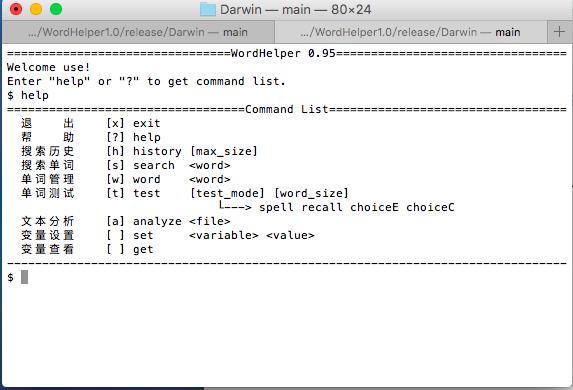
\includegraphics[keepaspectratio,width=\textwidth,height=0.75\textheight]{picture1.png} 

\section{搜索单词:}
\label{}

输入 \texttt{s $<$word$>$} 来搜索单词,如果您记不住单词的全拼,您可以输入部分字母以查询。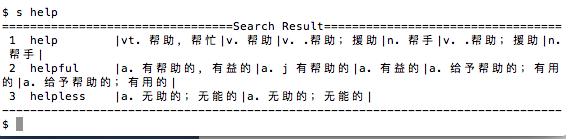
\includegraphics[keepaspectratio,width=\textwidth,height=0.75\textheight]{picture2.png}

\section{搜索历史:}
\label{}

如果您想查询历史纪录,请输入:\texttt{h [max\_size]}。 其中size代表您想查询的历史纪录数量. 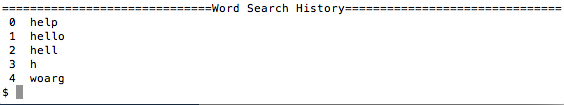
\includegraphics[keepaspectratio,width=\textwidth,height=0.75\textheight]{picture3.png}

\section{文本分析:}
\label{}

如果您想对一片英文文本进行分析,请输入:\texttt{a $<$file$>$}, 文本分析会自动帮您挑出高频词汇,生词还有不在词库中的单词。
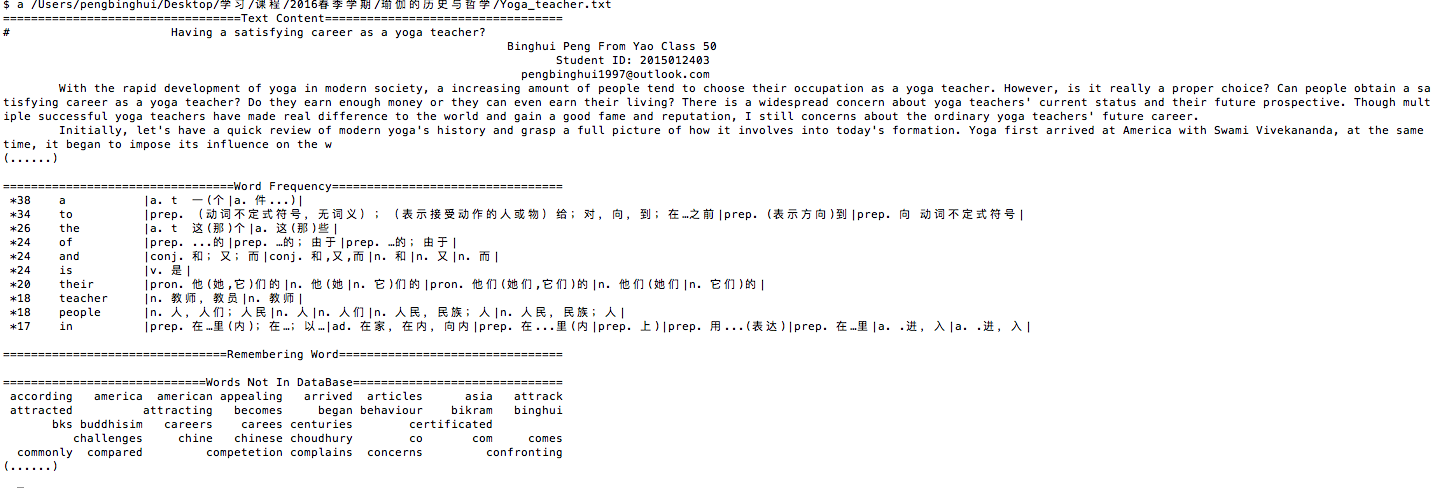
\includegraphics[keepaspectratio,width=\textwidth,height=0.75\textheight]{picture4.png}

\section{单词测试:}
\label{}

\subsection{选择模式:}
\label{}

如果您想单词测试,请输入\texttt{[t] [test\_mode] [word\_size]},目前我们有拼写,回忆,给中文选英文,给英文选中文四种模式,它们分别对应\texttt{spell}, \texttt{recall}, \texttt{choiceE}, \texttt{choiceC}.

\subsection{测试进行时}
\label{}

进入测试界面后,请您根据提示输入答案,每道题过后,系统会自动询问您是否继续测试,同时您也可以选择是否现实题目答案,具体命令如下:

\texttt{c}: Continue the test.

\texttt{a}: Show the correst answer.

\texttt{s}: Show the detail information about this word.

\texttt{m}: Enter into word manage interface.

\texttt{i}: Do not want to have this word tested anymore.

\texttt{?}: Get help information.

\texttt{x}: Exit test.
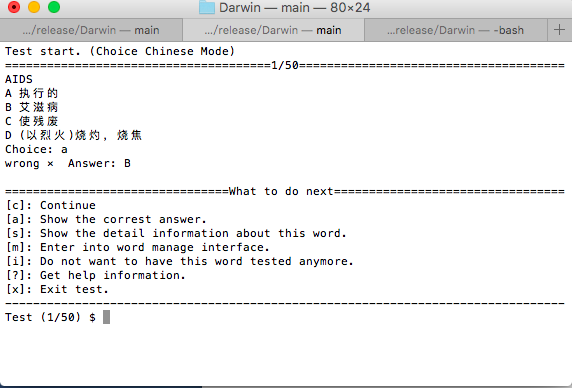
\includegraphics[keepaspectratio,width=\textwidth,height=0.75\textheight]{picture5.png}

\section{变量查看}
\label{}

您可以输入\texttt{get}来查看系统默认变量

\section{变量设置}
\label{}

您可以输入\texttt{set $<$variable$>$ $<$value$>$}来设置系统变量。
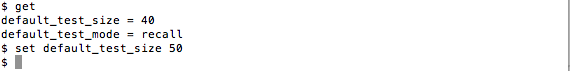
\includegraphics[keepaspectratio,width=\textwidth,height=0.75\textheight]{picture6.png}

\section{单词管理}
\label{}
\end{document}